\documentclass[tikz,border=3pt]{standalone}
\usepackage{pgfplots}
\usepgfplotslibrary{groupplots}
\pgfplotsset{compat=1.18}
\begin{document}
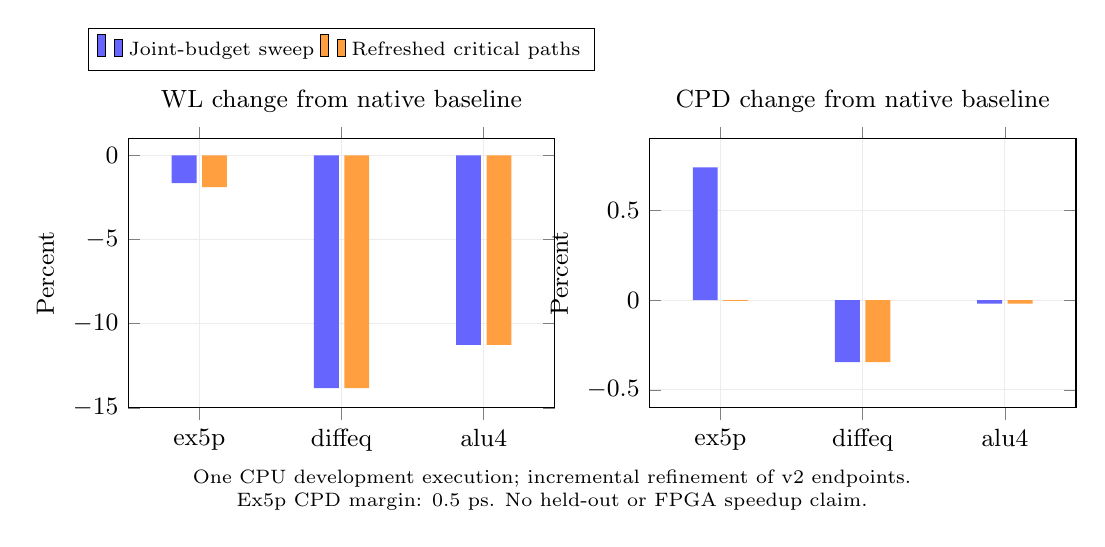
\begin{tikzpicture}
\begin{groupplot}[group style={group size=2 by 1,horizontal sep=1.2cm},width=7cm,height=5cm,ybar,/pgf/bar width=9pt,symbolic x coords={ex5p,diffeq,alu4},xtick=data,enlarge x limits=.25,grid=major,grid style={gray!15},tick label style={font=\small},label style={font=\small},title style={font=\small}]
\nextgroupplot[title={WL change from native baseline},ylabel={Percent},ymin=-15,ymax=1,legend style={font=\scriptsize,at={(.5,1.25)},anchor=south,legend columns=2}]
\addplot[fill=blue!60,draw=none] coordinates {(ex5p,-1.64442531) (diffeq,-13.82651492) (alu4,-11.26177024)};
\addplot[fill=orange!75,draw=none] coordinates {(ex5p,-1.87688334) (diffeq,-13.82651492) (alu4,-11.26177024)};
\legend{Joint-budget sweep,Refreshed critical paths}
\nextgroupplot[title={CPD change from native baseline},ylabel={Percent},ymin=-0.6,ymax=0.9,legend style={font=\scriptsize,at={(.5,1.25)},anchor=south,legend columns=2}]
\addplot[fill=blue!60,draw=none] coordinates {(ex5p,0.73949355) (diffeq,-0.34478807) (alu4,-0.01923613)};
\addplot[fill=orange!75,draw=none] coordinates {(ex5p,-0.00478327) (diffeq,-0.34478807) (alu4,-0.01923613)};
\end{groupplot}
\node[anchor=north,font=\scriptsize,align=center] at (current bounding box.south) {One CPU development execution; incremental refinement of v2 endpoints.\\Ex5p CPD margin: 0.5 ps. No held-out or FPGA speedup claim.};
\end{tikzpicture}
\end{document}
